\documentclass{article}

\usepackage{graphicx}
\usepackage{float}
\graphicspath{ {./images/} }

\title{Altitude-Cognizant Scalar Slepian Functions}
\author{H. A. Werth}
\date{}


\setlength{\parskip}{0.5cm plus4mm minus3mm}

\textwidth=6.4in
\textheight=8.5in
\hoffset=-0.7in
\voffset=-0.7in

\setlength{\parindent}{0cm} 

\setcounter{section}{-1}

\begin{document}
\maketitle

\tableofcontents 


\section{Introduction: description of task}

The scalar spherical harmonics are a family of real-valued functions which provide a basis in spherical coordinates for real-valued functions defined on the sphere of unit radius. In this context, to be defined on the unit sphere is to be a function of the position of the radial vector \textbf{r}. Scalar Slepian functions are specialized linear combinations of these spherical harmonics. They form an alternative basis, so that any function expressible as a combination of spherical-harmonics may be rewritten in terms of the Slepian functions. 

While the spherical harmonics are a global basis, in the sense that they may be used to express functions on their whole domain, the Slepian functions are computed locally in order to represent functions on a region $R$ of the sphere. The utility of the Slepian basis is in that, for a chosen region and a chosen bandwidth, they are the most concentrated within each. (For a proof (?) of this, see [Simons 2006].) The limitation of the bandwidth is a condition on the number of spherical harmonics used in each function, an important consideration in computation. Since a Slepian function is a linear combination of spherical harmonics, to "compute/construct a Slepian function" is to solve for a vector of spherical-harmonic coefficients.

The Slepian functions are designed to represent and analyse experimental data. In this document we will be concerned with locally-collected satellite data which are values of the negative first derivative of some potential field on a planet's surface. The task of interest is data inversion -- we want to use the radial derivative data to solve for the potential field, which is mathematically approximated by a real-valued function of radial position. Since we assume the data are available only regionally, we aim to represent (a local portion of) the potential field as a linear combination of Slepian functions. So, to "solve/invert for the potential field" is, in practice, to determine a vector of coefficients in the Slepian basis.

The Slepian functions we will be using are "altitude-cognizant". They are best-concentrated like the classical Slepian functions, but their construction explicitly takes into account the fact that the data are recorded above the source of the potential field. One solves for the spherical-harmonic coefficients of the Slepian basis functions under the assumption that the coefficients are elevated to the average altitude of data collection. The data inversion process involves first representing the potential field at the level of the data and then "downward continuing" that representation to the planet's surface. For a detailed account of both the derivation and application of the altitude-cognizant Slepian functions, see [Plattner and Simons 2017]. 

The purpose of this document is to present the matlab code for all the steps of the data inversion process, from generating random data to solving for the potential field.

\section{Create model potential field}

We need to base our creation of random data on a model potential field, so that we may compare the inverted potential field to this model field in the final step.

\vspace{3mm}

\setlength{\parskip}{.1mm}

Create field:

\vspace{3mm}

\verb!Lmax=20 !

\verb!rnd_lmcosi=plm2rnd(Lmax,0);!

\verb!coef=lmcosi2coef(rnd_lmcosi);!

\setlength{\parskip}{0.5cm plus4mm minus3mm}

The "field" is a linear combination of spherical harmonics, whose coefficients are given in the matrix output \verb!coef!.

\vspace{3mm}

\setlength{\parskip}{.1mm}

Plot field:

\vspace{3mm}

\verb!lmcosi=coef2lmcosi(coef/sqrt(4*pi));!

\verb!clf; !

\verb!res = 0.5; !

\verb!plotplm(lmcosi,[],[],2,res)!

\verb!title('True potential on planet surface')!

\verb!cax=caxis!

\verb!caxis([-1 1]*max(abs(cax)))!

\verb!kelicol(1)!

\verb!colorbar !

\setlength{\parskip}{0.5cm plus4mm minus3mm}

It is necessary to include the factor \verb!sqrt(4*pi)! whenever plotting fields generated with \verb!plm2rnd! using \verb!plotplm!.

\begin{figure}[H]
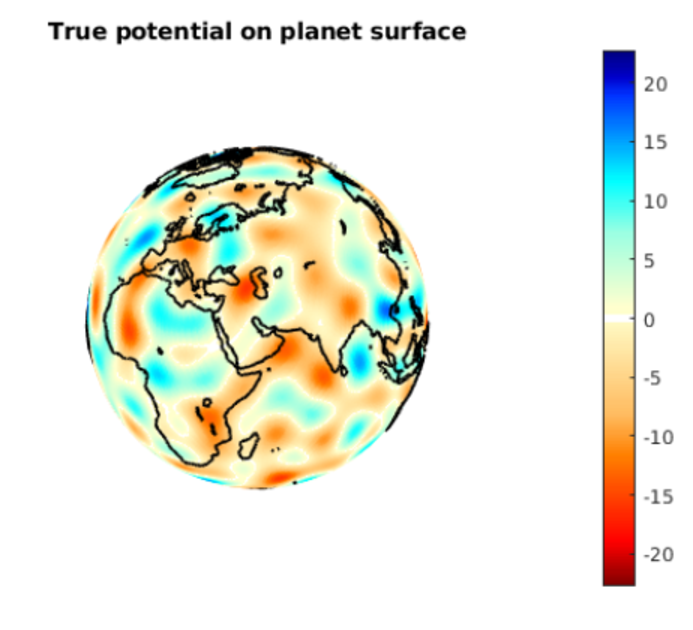
\includegraphics[scale=.6]{true_potential}
\end{figure}

\section{Evaluate the field's derivative at random points}

Choose parameters for data location:

\vspace{3mm}

\setlength{\parskip}{.1mm}

\verb!dom= 'africa'!

\verb!N= 2000 ! 

\verb!planetrad=6371!

\verb!satrad=6371+400!

\verb!varalt= 100!

\setlength{\parskip}{0.5cm plus4mm minus3mm}

\verb!N! is the maximum number of data points. Each datum is recorded at a satellite altitude; \verb!satrad! is the average of these altitudes.  \verb!varalt! is the optional range of variation for satellite altitude.

\vspace{3mm}

Get random data locations:

\vspace{3mm}

\setlength{\parskip}{.1mm}

\verb![lon, lat] = randinpoly(dom,N);!

\verb!cola = 90-lat!

\verb!rad = satrad +(rand(length(lon),1)-0.5)*varalt;!

\verb!theta= cola*pi/180!

\verb!phi = lon*pi/180!

\setlength{\parskip}{0.5cm plus4mm minus3mm}

This sequence of steps generates up to \verb!N! random points first within \verb!dom!, and then, for each point, generates a random satellite altitude which has a uniformly random distribution in  \verb![satrad-varalt/2 satrad+varalt/2]!.

\vspace{3mm}

Evaluate the derivative at random points:

\verb!data=rGscal(coef,theta,phi,rad,planetrad)';!

\setlength{\parskip}{0.5cm plus4mm minus3mm}

The function \verb!rGscal! computes and evaluates the field's negative radial derivative point-wise, taking into account the altitude of the points. The values contained in the output matrix \verb!data! form our "collected data".


\subsection{Compute spherical-harmonic coefficients of Slepian basis functions}


\verb![G,V]=glmalphaup(dom,Lmax,satrad,planetrad);!

\setlength{\parskip}{0.5cm plus4mm minus3mm}

The altitude-cognizant Slepian basis functions depend on \verb!data! only through the region \verb!dom! and the average altitude \verb!satrad! of their collection. \verb!G! is the matrix of coefficients and \verb!V! the vector of eigenvalues (for more information on the output of \verb!glmalphaup!, refer to its \verb!help! section).

This step is relegated to a subsection because it is not necessary to perform in the course of data inversion. The function \verb!LocalIntField!, used in the next section, computes the appropriate Slepian basis automatically.

\section{Solve for the potential field}

\vspace{3mm}

\setlength{\parskip}{.1mm}

\verb!J=40!

\verb!result_coef=LocalIntField(data,rad,theta,phi,dom,Lmax,J,planetrad,satrad);!


\setlength{\parskip}{0.5cm plus4mm minus3mm}


The choice of \verb!J! dictates how many of the Slepian basis functions are used to represent the potential field in the inversion, which the function \verb!LocalIntField! wholly accomplishes. Larger \verb!J! means the computation is more sensitive to noise but results in higher spatial resolution.

Plot inverted field:

\vspace{3mm}

\setlength{\parskip}{.1mm}

\verb!figure!

\verb!result_lmcosi=coef2lmcosi(result_coef/sqrt(4*pi));!

\verb!plotplm(result_lmcosi,[],[],2,res)!

\verb!title('Inverted potential on planet surface from radial derivative data')!

\verb!caxis([-1 1]*max(abs(cax)))!

\verb!kelicol(1)!

\verb!colorbar !

\begin{figure}[H]
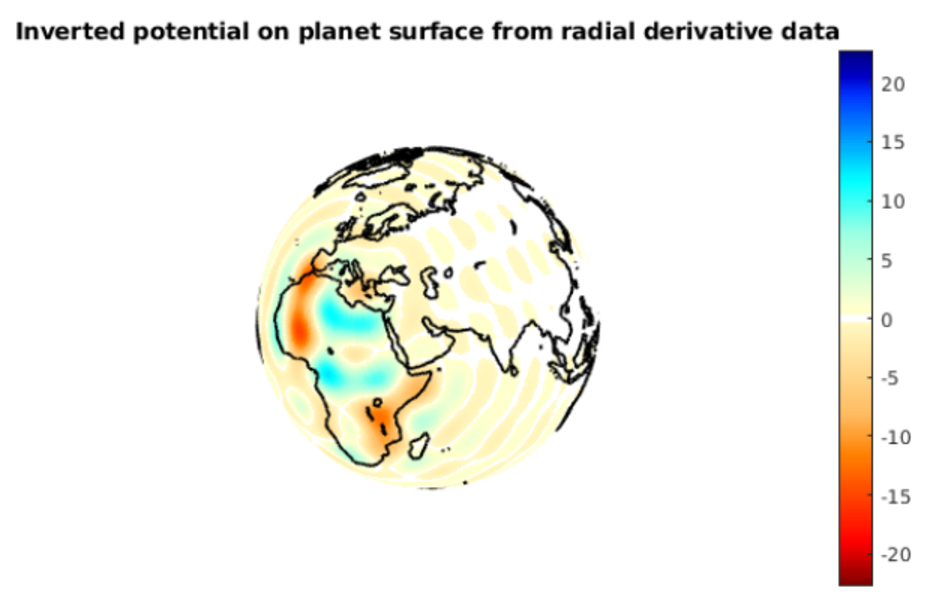
\includegraphics[scale=.6]{inverted_potential}
\end{figure}

\setlength{\parskip}{0.5cm plus4mm minus3mm}

In order to plot, we had first to convert the coefficients to \verb!lmcosi! format, as usual. Note how the inverted field is expressed in the local basis while the true field with which we began was in the global basis.


Plot difference of true and inverted field:


\vspace{3mm}

\setlength{\parskip}{.1mm}

\verb!clf;!

\verb!diff_lmcosi=coef2lmcosi((coef - result_coef)/sqrt(4*pi));!

\verb!plotplm(diff_lmcosi,[],[],2,res)!

\verb!title('Difference between true and inverted potential fields')!

\verb!caxis([-1 1]*max(abs(cax)))!

\verb!kelicol(1)!

\verb!colorbar !

\begin{figure}[H]
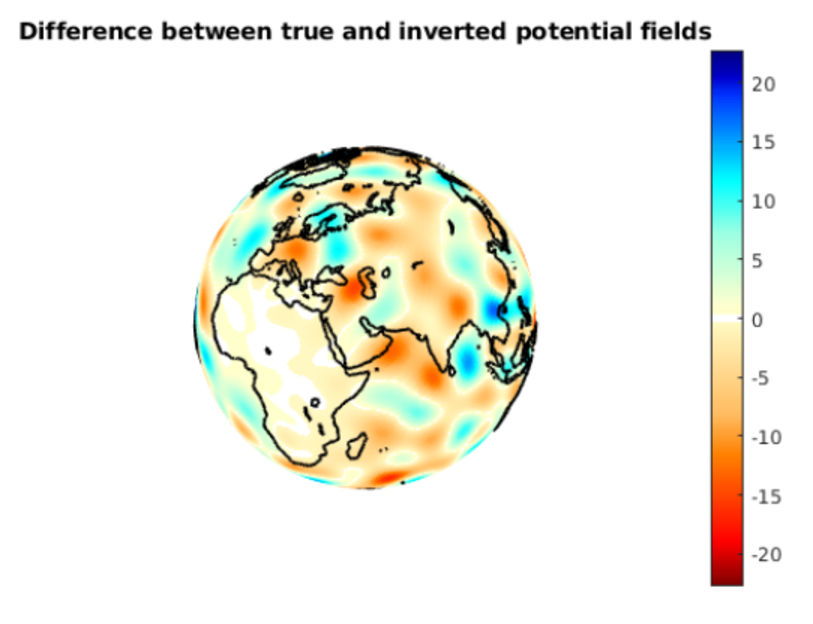
\includegraphics[scale=.65]{difference_potential}
\end{figure}

\end{document}